\label{ch:3}
To study the dynamics of the system, we need to consider the complete diffusion equation, along with the Poisson equation. The Poisson equation depends on the concentration of the different electrolyte species. Since the concentrations vary with time, the Poisson equation changes for every time step. The system we are dealing with is

\begin{align}
\frac{\partial C_+}{\partial t} &= D_+ \left(\nabla^2 C_+ -  \nabla (C_+ \nabla \Psi) \right) , \\
\frac{\partial C_-}{\partial t} &= D_- \left(\nabla^2 C_- + \nabla (C_- \nabla \Psi) \right), \\
\nabla^2 \Psi &= -\kappa^2 \left(C_+ - C_- \right).
\label{eq:dynamic-system-0}
\end{align}

subject to the following initial conditions
\begin{align}
C_+(t = 0, x) & = 0,\\
C_-(t = 0, x) & =  0,\\
\Psi(t = 0, x) &= 0.
\end{align}

where the super-script $SS$ indicates the steady state solution (See \ref{ch:2}). Here, $C_\pm$ are the concentrations for each species and $\Psi$ is the dimensionless electric potential defined in \ref{eq:dimensionless-potential}. Boundary conditions are given by

\begin{align}
\label{eq:1d-bondary}
C_s(\delta, t) = C_b,\\
J_s(0,t) = D_s\frac{\partial C_s}{\partial x}\big|_{x=0} = r\delta_{+,s},
\label{eq:diffusion-bc}
\end{align}

where $J_s(x,t)$ is the flux for each species and $\delta_{+,s}$ is the Kronecker delta and $s = \pm$. The delta is responsible for a non-zero boundary condition at the interface only for the interacting species (copper, in our case).

In order to build and test an algorithm which numerically approximates the solution to system \ref{eq:dynamic-system-0}, we start out with the diffusion problem in one dimension, without any reaction at the interface. We will start increasing the complexity of our problem until we solve system \ref{eq:dynamic-system-0} completely.

\section{Diffusion Only}

As a first approach to our problem, we evaluate the simpler diffusion-only problem



\begin{align}
\frac{\partial C}{\partial t} &= D \nabla^2 C,\\
\label{eq:diffusion}
\end{align}

which in our limit (infinite plate) we can write as


\begin{align}
\label{eq:diffusion-1d-1}
\frac{\partial C}{\partial t} &= D\frac{\partial^2 C}{\partial x^2}.\\
\end{align}

Here, $C$ stands for the concentration of a given species and $\mathcal{D}$ is the diffusion coefficient for that same species. The equation is subject to the following boundary conditions

\begin{align}
	C(t, x = \delta) = C_b,\\
	J(t, x = 0) = 0,
\end{align}

with

\begin{align}
	J(t, x) =-\mathcal{D}\frac{\partial C}{\partial x} 
\end{align}

 The initial condition for our system is

\begin{align}
	C(t = 0, x) = 0.
\label{eq:diffusion-initial-condition--diffonly}
\end{align}

In this section, we have solved the diffusion only problem. That is, we want to solve equation \ref{eq:diffusion-1d-1} considering in turn a zero flux boundary condition at $x=0$ ($s=-$), given by \ref{eq:1d-bondary}. It is found that the analytic solution to this problem by means of the separation of variables method is

\begin{align}
	\label{eq:solution-diffusion-1}
	C(x,t) = C_b\qty{1-\frac{4}{\pi} \sum_n \frac{(-1)^m}{(2m+1)}\exp\qtys{-\qty{\frac{(2n+1)\pi}{2}}^2\frac{D_- t}{\delta^2}}\cos\qty{\frac{(2m+1)\pi}{2} \frac{x}{\delta}}}.
\end{align}

The analytic solution \ref{eq:solution-diffusion-1} worked out in Appendix \ref{appendix:analytic-diff-only} and the numerical solution is described in \ref{appendix:numerical-solution-diffusion-only}. Results are shown in \ref{fig:diffusion-comparison}.

As it can be seen in Fig. \ref{fig:diffusion-comparison}, the analytic and the numeric results match closely for every time step plotted, which gives us a green light to keep adding complexity to our system.
 
\begin{figure}[htbp]
\centering
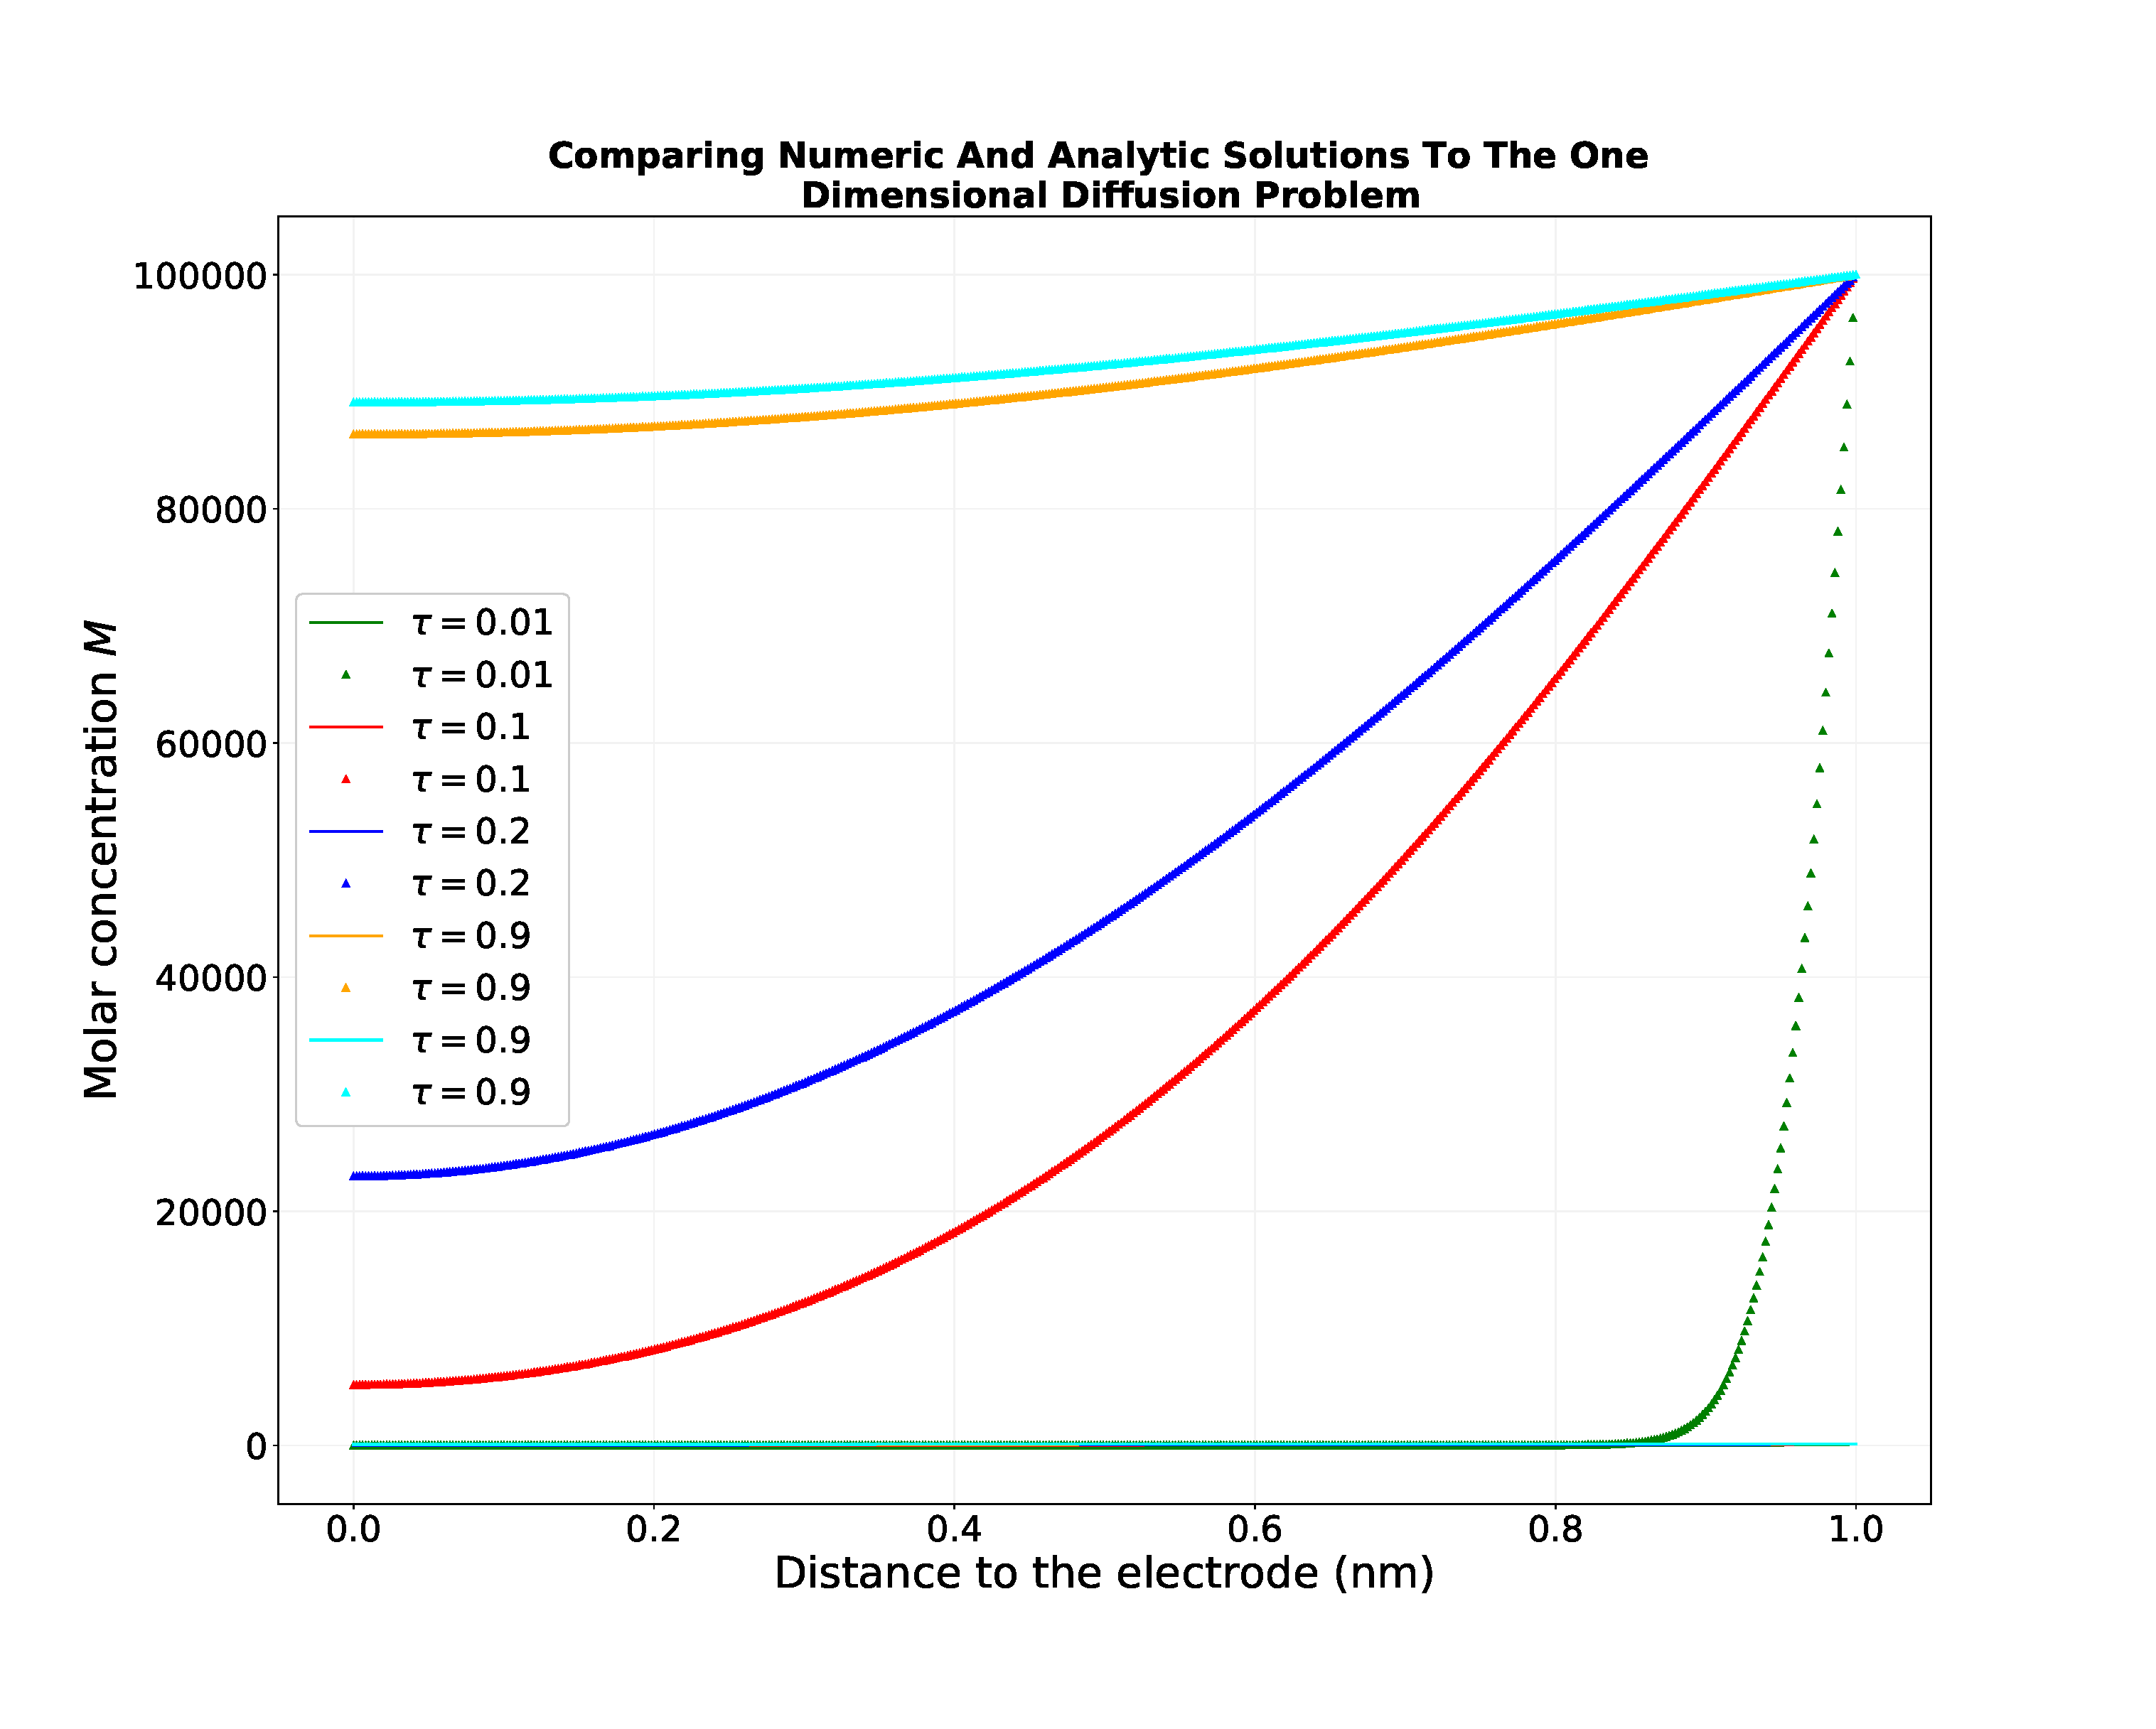
\includegraphics[width=\textwidth]{concentration-diffusiononly-comparison}
\caption{Each curve represents the concentration profile at increasingly large $t$. Continuos lines represent the analytic solution at each time step and the discrete markers listed in the image legend are represent the numerical solution. Steady State in the diffusion-only problem will be when concentration is $C_b=1M$ throughout the domain.}
\label{fig:diffusion-comparison}
\end{figure}


\newpage
